% !TeX root = ../../Parte2.tex
\secmeme{css/misure}
\section{Dimensioni}

\begin{frame}{Box model}\transfade\centering
  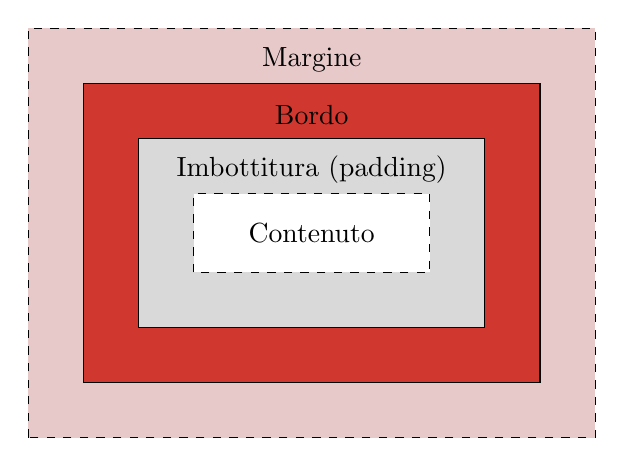
\begin{tikzpicture}

    \draw[fill=red!40!gray!30!white, dashed] (-3.6,-2.6) rectangle (3.6,2.6);
    \draw[fill=brown!20!red!70!gray] (-2.9,-1.9) rectangle (2.9,1.9);
    \draw[fill=gray!30!white] (-2.2,-1.2) rectangle (2.2,1.2);
    \draw[fill=white, dashed] (-1.5,-.5) rectangle (1.5,.5);

    \draw (0,2.2) node {Margine};
    \draw (0,1.5) node {Bordo};
    \draw (0,.8) node {Imbottitura (padding)};
    \draw (0,0) node {Contenuto};

  \end{tikzpicture}\\
\end{frame}

\begin{frame}[fragile]{Dimensione contenuto}\transfade\centering
  \begin{minted}[firstline=2, lastline=9, fontsize=\normalsize]{css}
p{
    width: 100px;
    height: auto;

    min-width: 100%;
    min-height: 100pt;

    max-width: 100px;
    max-height: 100px;
}
  \end{minted}
\end{frame}
\begin{frame}[fragile]{Bordo}\transfade\centering
  \htmlDual[-s A7][][trim={0 7cm 0 0},clip][css]{<style>}{
  p.solid {border-style: solid;}
  p.dotted {border-style: dotted;}
  p.dashed {border-style: dashed;}
  p.double {border-style: double;}
  p.none {border-style: none;}
  p.hidden {border-style: hidden;}}{
  </style>
  <p class="solid">Bordo normale.</p>
  <p class="dotted">Bordo puntinato.</p>
  <p class="dashed">Bordo trateggiato.</p>
  <p class="double">Bordo doppio.</p>
  <p class="none">Senza bordo.</p>}\pause\bigskip
  \begin{minted}[firstline=2, lastline=6, fontsize=\normalsize]{css}
    p{
border-width: 5px /*o thin, medium, thick */;
border-color: orange;

border: 5px solid green; /* scorciatoia */
/* border-left, border-right, border-top, border-bottom */
    }
      \end{minted}
\end{frame}

\begin{frame}[fragile]{Bordo tabelle}\transfade\centering
  \htmlDual[-s A7][][trim={0 7cm 4cm 0},clip][css]{<style>}{
  #tab1, #tab1 th, #tab1 td{
    border: 1px solid black;
  }

  #tab2, #tab2 th, #tab2 td{
    border: 1px solid black;
    border-collapse: collapse;
  }
  }{
  </style>
  <table id=tab1><tr><td>1<td>2<tr><td>3<td>4</table><br>
  <table id=tab2><tr><td>1<td>2<tr><td>3<td>4</table>}
\end{frame}